\documentclass{article}

\usepackage{fancyhdr}
\usepackage[includeheadfoot,left=1in, right=0.5in, top=0.5in, bottom=0.5in]{geometry}
\usepackage{lastpage}
\usepackage{extramarks}
\usepackage[usenames,dvipsnames]{color}
\usepackage{graphicx}
\usepackage{listings}
\usepackage{courier}
\usepackage{tikz}
\usepackage{color}
\usepackage{float}
\usepackage{url}
\usepackage{subfigure}
\usepackage{varwidth}
\usepackage{caption}
\usepackage{multirow}
\usepackage[pdfborder={0 0 0}]{hyperref}
\usepackage[compact,small]{titlesec}
\usepackage{microtype}
\usepackage{verbatim}
\usepackage{booktabs}
\usepackage{indentfirst}

\parskip = 0.5\baselineskip
\setlength{\belowcaptionskip}{-\baselineskip}

\captionsetup{font=scriptsize}
\captionsetup{labelfont=bf}

\pagestyle{fancy}
\rhead{Max Thrun}
\lhead{EECE6080 - HW 4}
\rfoot{Page\ \thepage\ of \protect\pageref{LastPage}}
\cfoot{}
\renewcommand\headrulewidth{0.4pt}
\renewcommand\footrulewidth{0.4pt}

% make verbatim text small
\makeatletter
\g@addto@macro\@verbatim\small
\makeatother

\setlength\parindent{0pt} % Removes all indentation from paragraphs

\definecolor{sh_comment}{rgb}{0.12, 0.38, 0.18 } %adjusted, in Eclipse: {0.25, 0.42, 0.30 } = #3F6A4D
\definecolor{sh_keyword}{rgb}{0.37, 0.08, 0.25}  % #5F1441
\definecolor{sh_string}{rgb}{0.06, 0.10, 0.98} % #101AF9

\lstset{
    language=vhdl,
    xleftmargin=.25in,
    xrightmargin=.25in,
    numbers=left,
    numberstyle=\tiny,
    frame=tb,
    showstringspaces=false,
    captionpos=b,
    stringstyle=\color{sh_string},
    keywordstyle = \color{sh_keyword}\bfseries,
    commentstyle=\color{sh_comment}\itshape,
    basicstyle=\small\sffamily,
    %numbersep=-5pt,
    belowskip=\baselineskip,
    aboveskip=\baselineskip
}

\title{
    \vspace{2in}
    \textmd{\textbf{EECE6080 - HW 4}}\\
    \vspace{4in}
}
\author{\textbf{Max Thrun}}

\begin{document}
\maketitle

\begin{figure}[H]
    \centering
    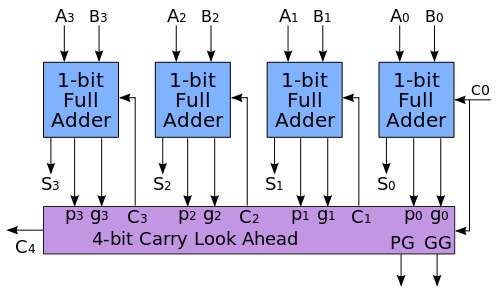
\includegraphics[width=\linewidth]{../4-bit_carry_lookahead_adder.png}
    \caption{Carry Chain Design}
\end{figure}

\begin{figure}[H]
    \centering
    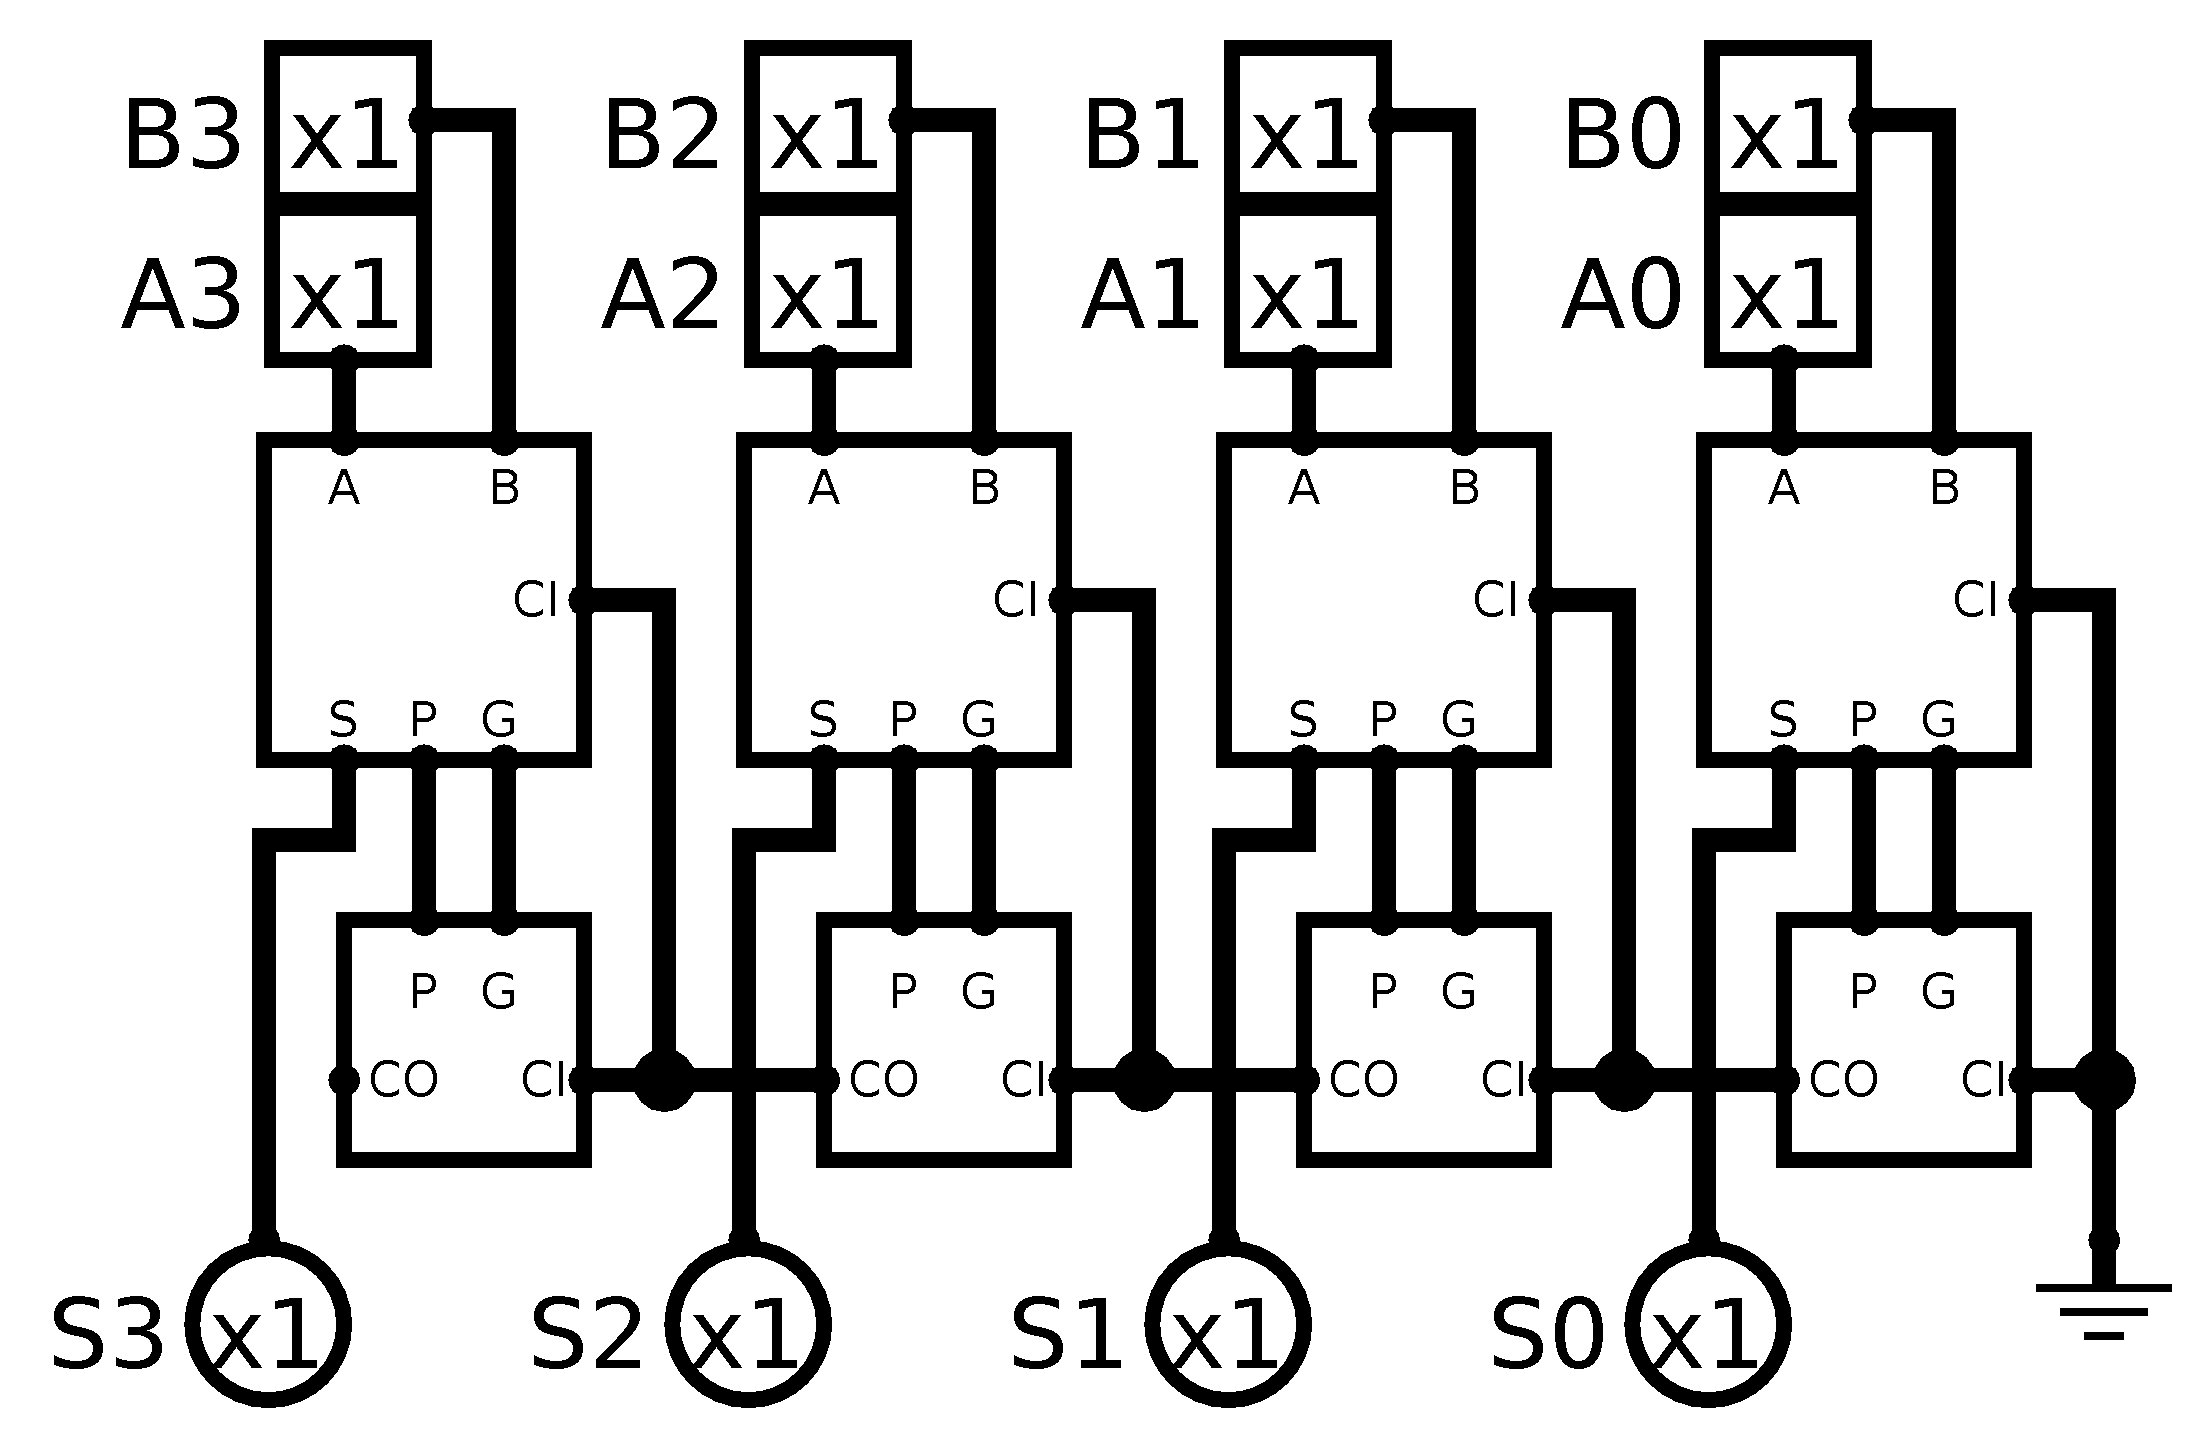
\includegraphics[width=\linewidth]{../logisim_top.png}
    \caption{Top Level Design}
\end{figure}

\begin{figure}[H]
    \centering
    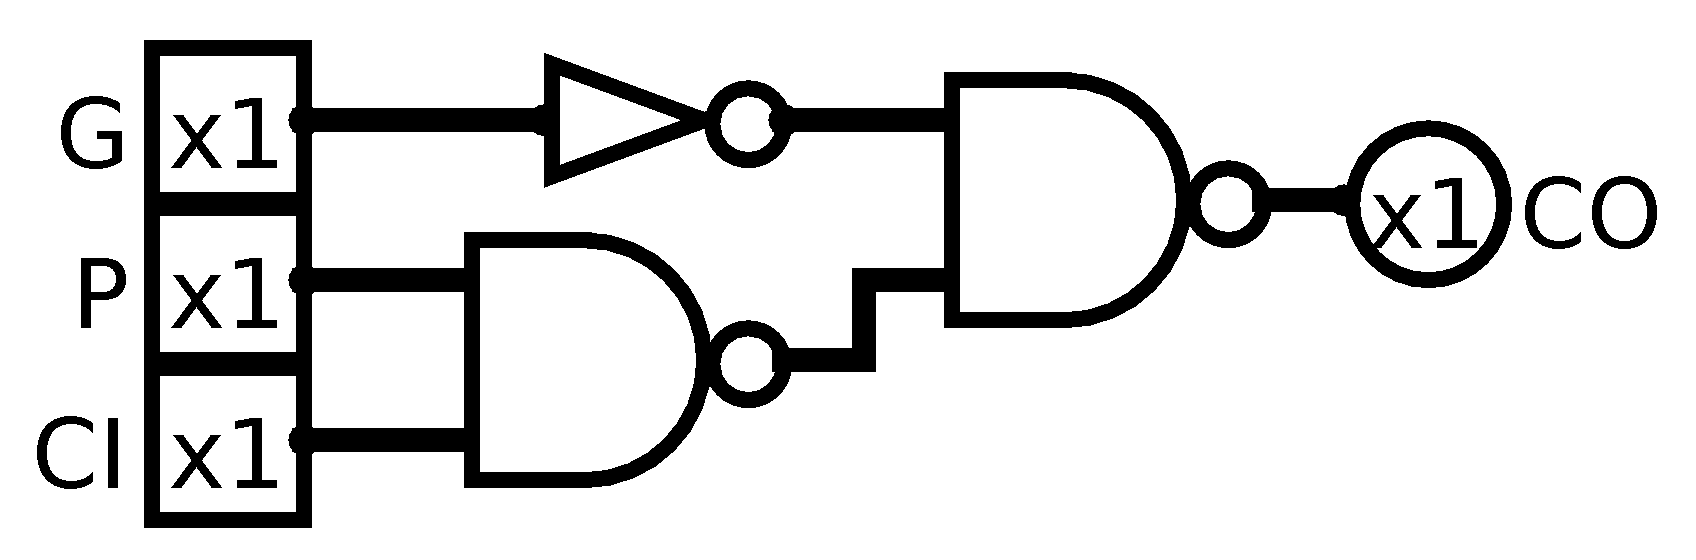
\includegraphics[width=\linewidth]{../logisim_carry_slice.png}
    \caption{1-Bit Carry Design}
\end{figure}

\begin{figure}[H]
    \centering
    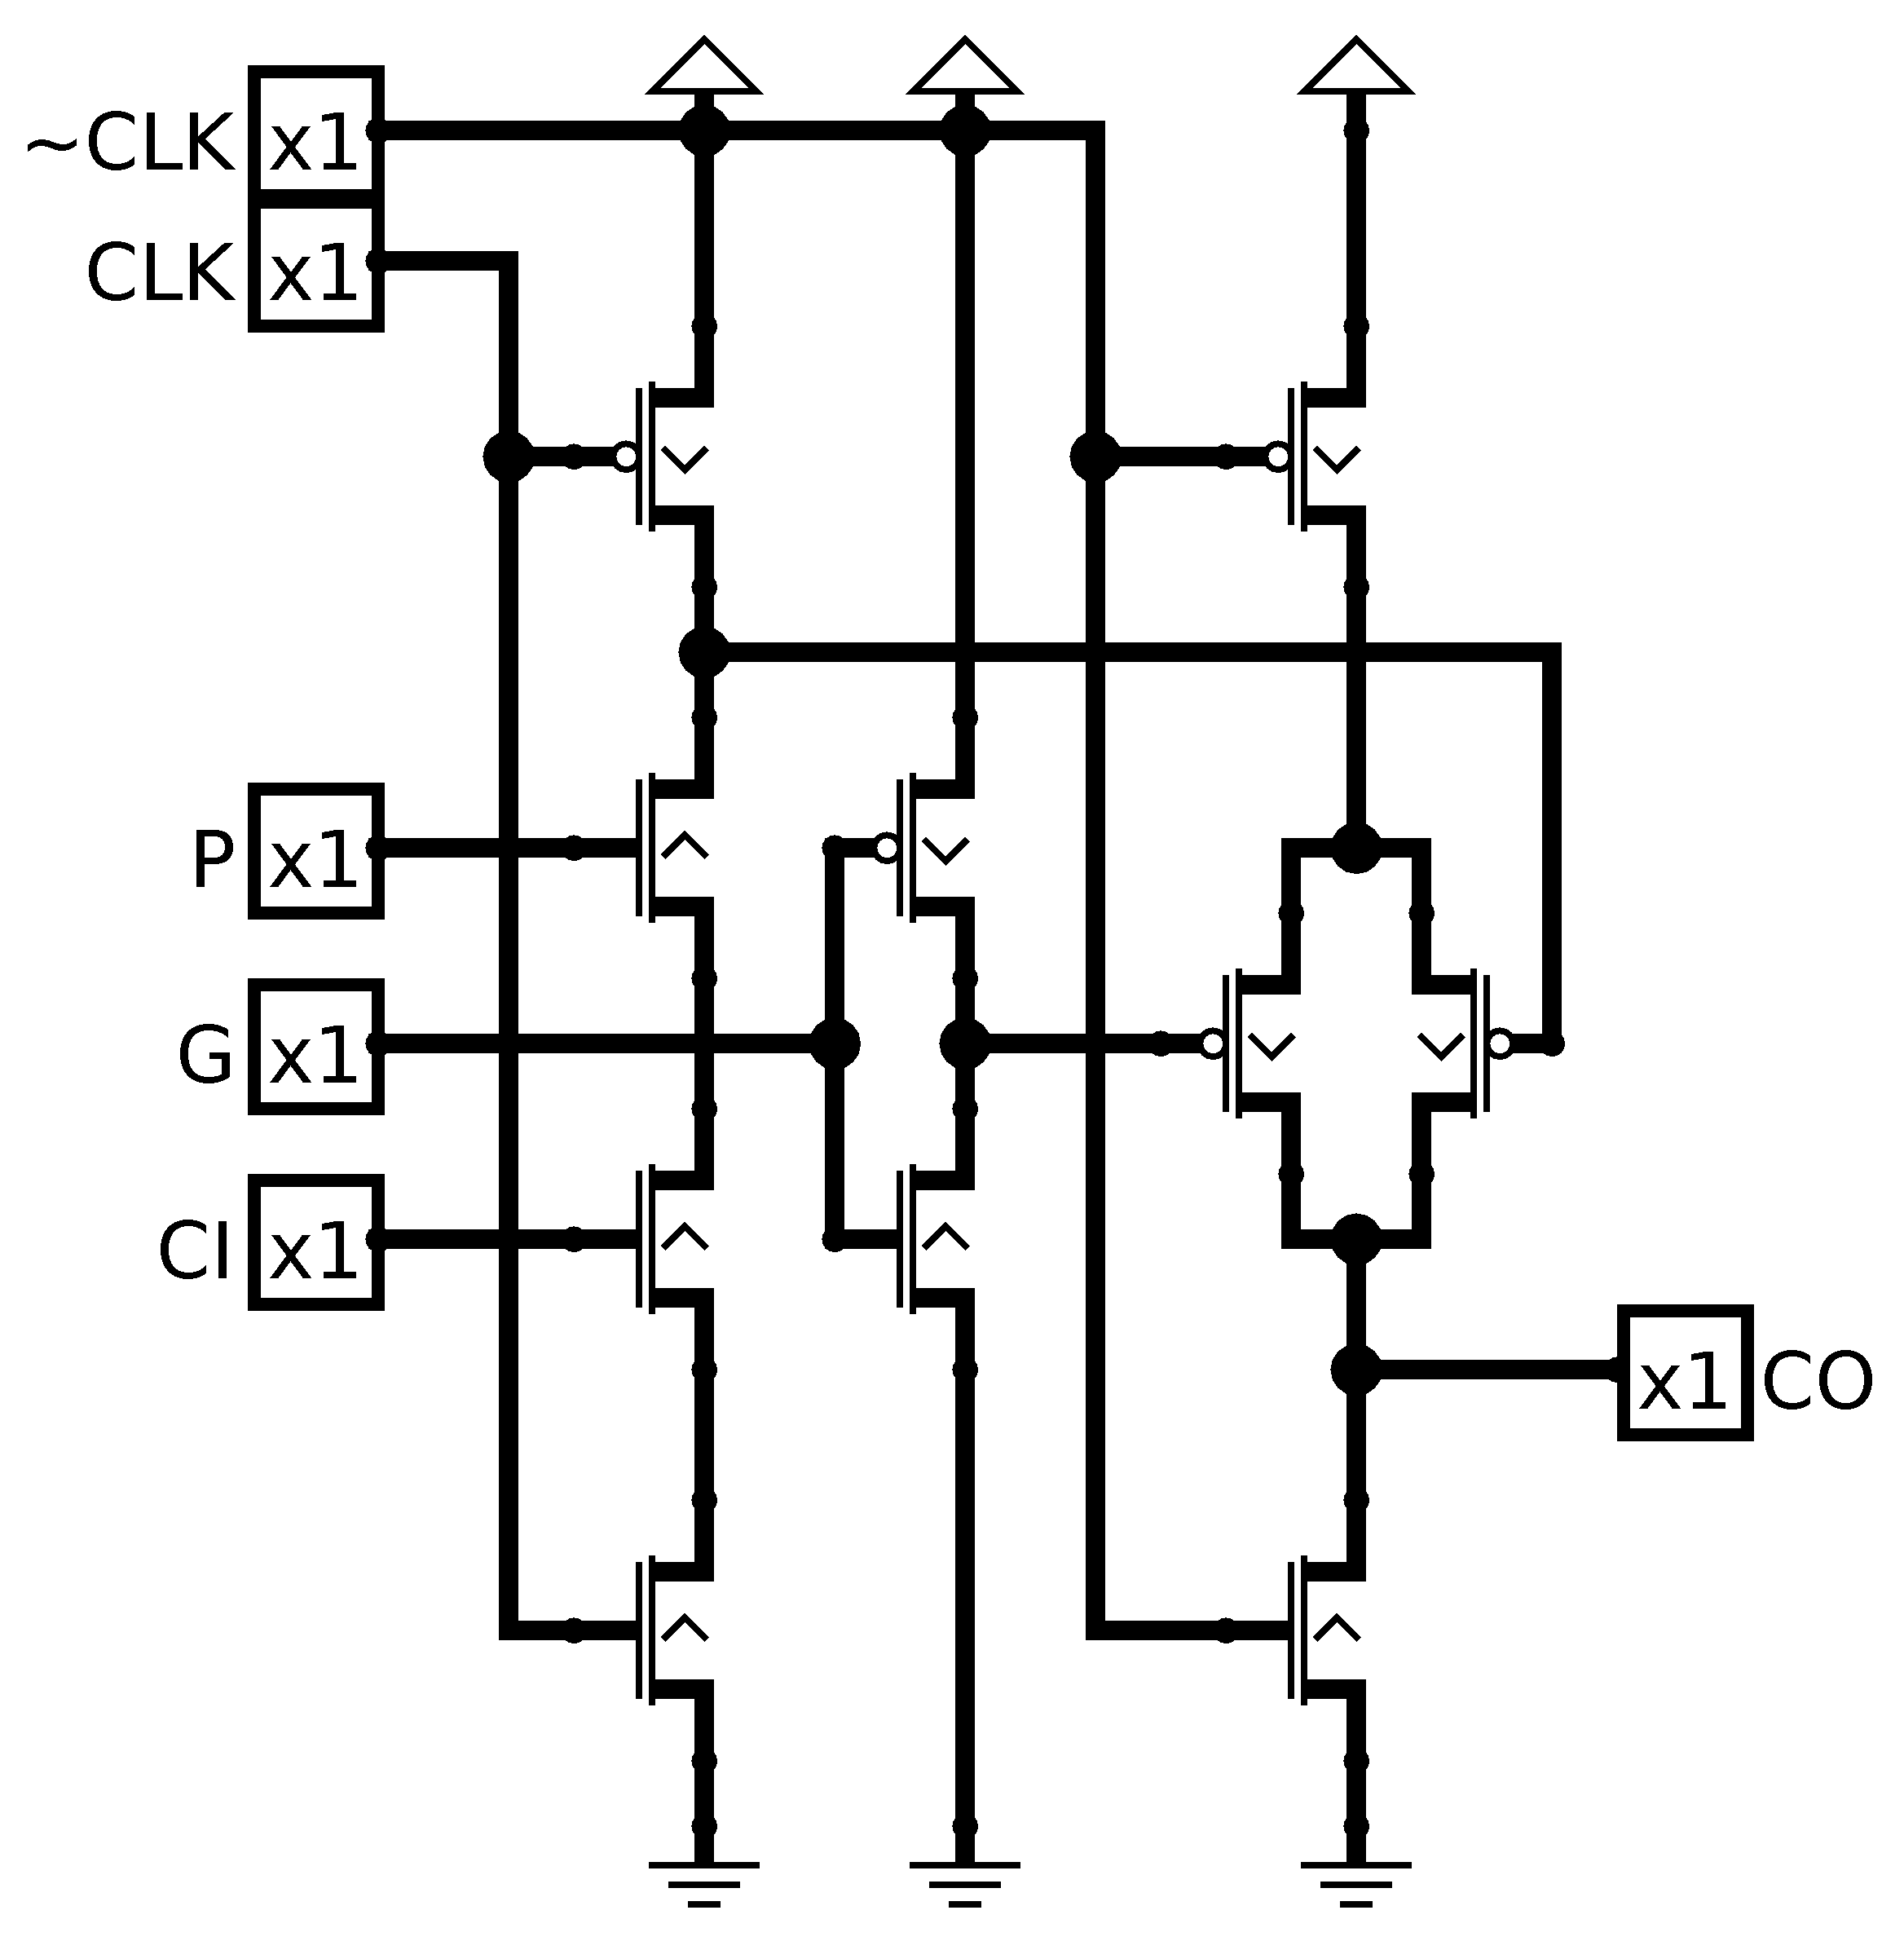
\includegraphics[width=\linewidth]{../logisim_carry_slice_fets.png}
    \caption{1-Bit Carry Design CMOS}
\end{figure}

\newpage
\subsection*{Part 1}

\lstinputlisting[caption=Inverter]{../part_1_inv.sp}
\lstinputlisting[caption=P NAND]{../part_1_p_nand.sp}
\lstinputlisting[caption=N NAND]{../part_1_n_nand.sp}
\lstinputlisting[caption=Library]{../../models/library.sp}

\begin{figure}[H]
    \centering
    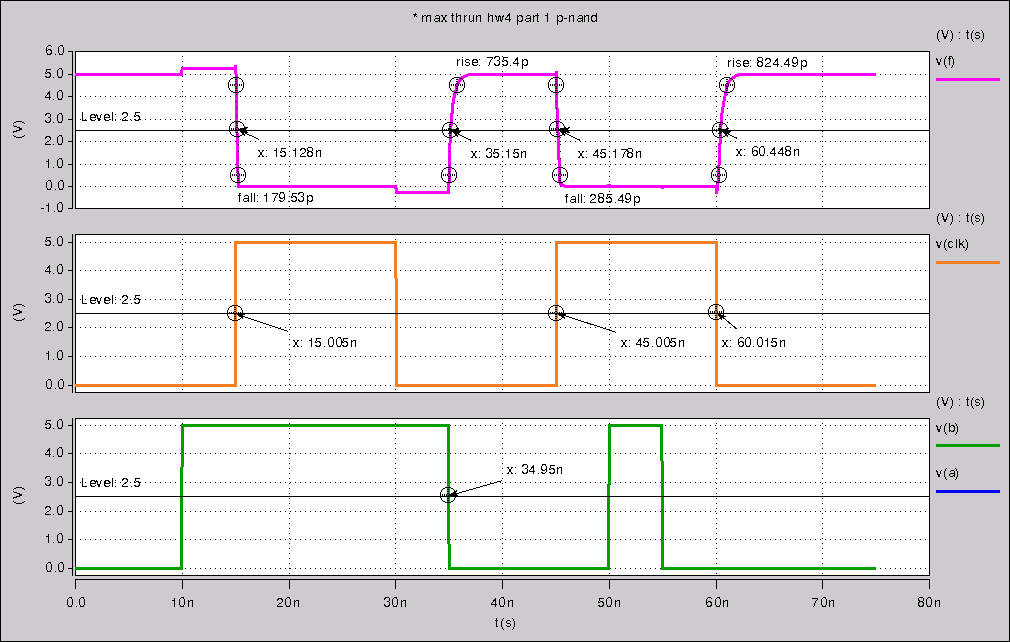
\includegraphics[width=\linewidth]{../part_1_p_nand.png}
    \caption{Part 1 P NAND Simulation Result}
\end{figure}

\begin{figure}[H]
    \centering
    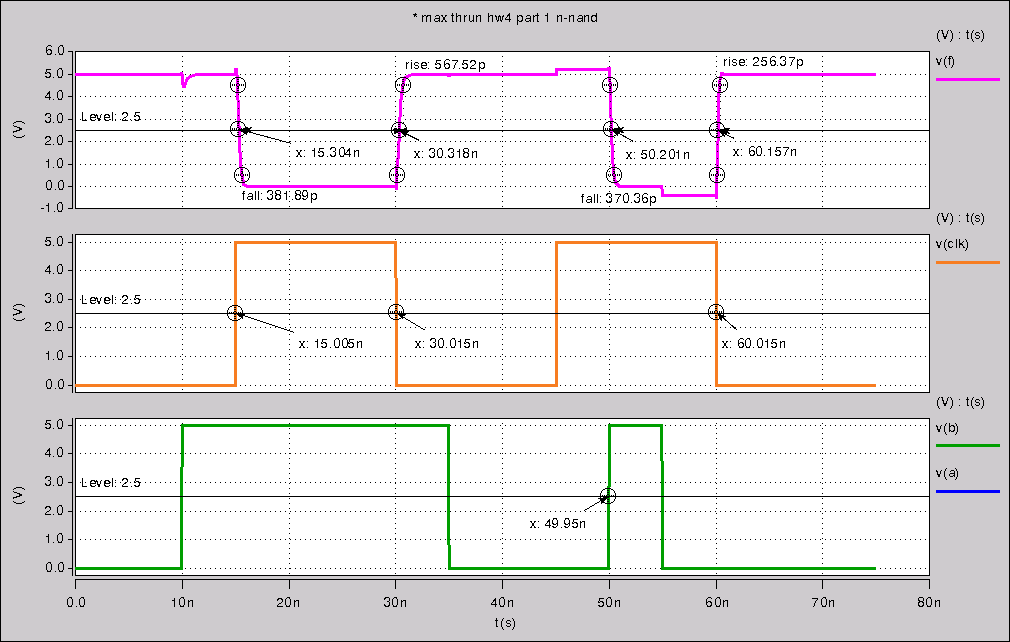
\includegraphics[width=\linewidth]{../part_1_n_nand.png}
    \caption{Part 1 N NAND Simulation Result}
\end{figure}

\begin{figure}[H]
    \centering
    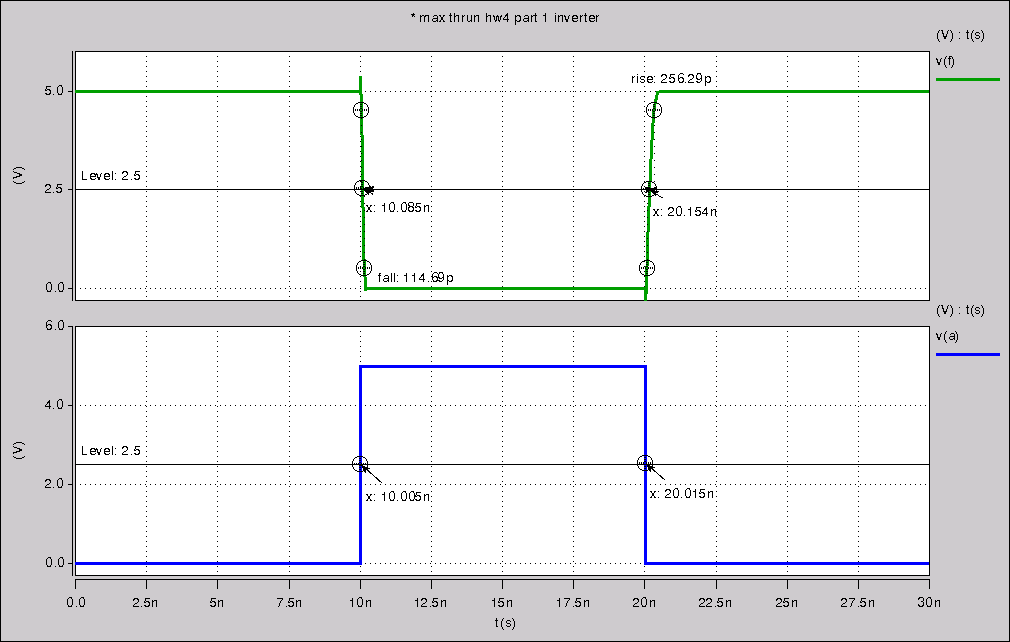
\includegraphics[width=\linewidth]{../part_1_inv.png}
    \caption{Part 1 Inverter Simulation Result}
\end{figure}

\newpage
\subsection*{Part 2}

\lstinputlisting[caption=Part 2 Spice File]{../part_2.sp}

\begin{figure}[H]
    \centering
    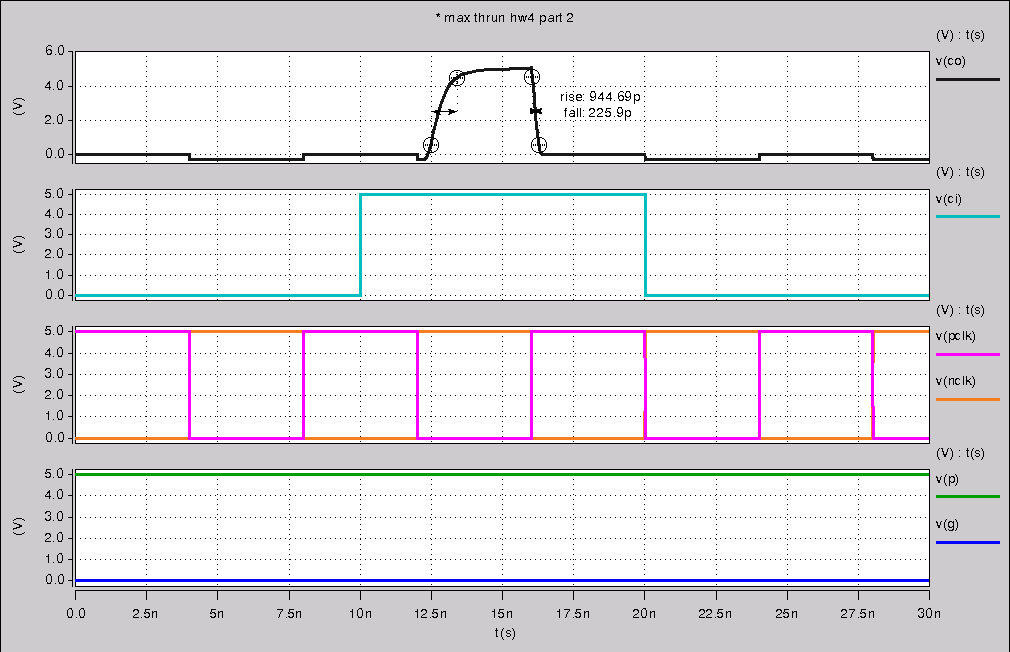
\includegraphics[width=\linewidth]{../part_2.png}
    \caption{Part 2 Simulation Result}
\end{figure}

\begin{figure}[H]
    \centering
    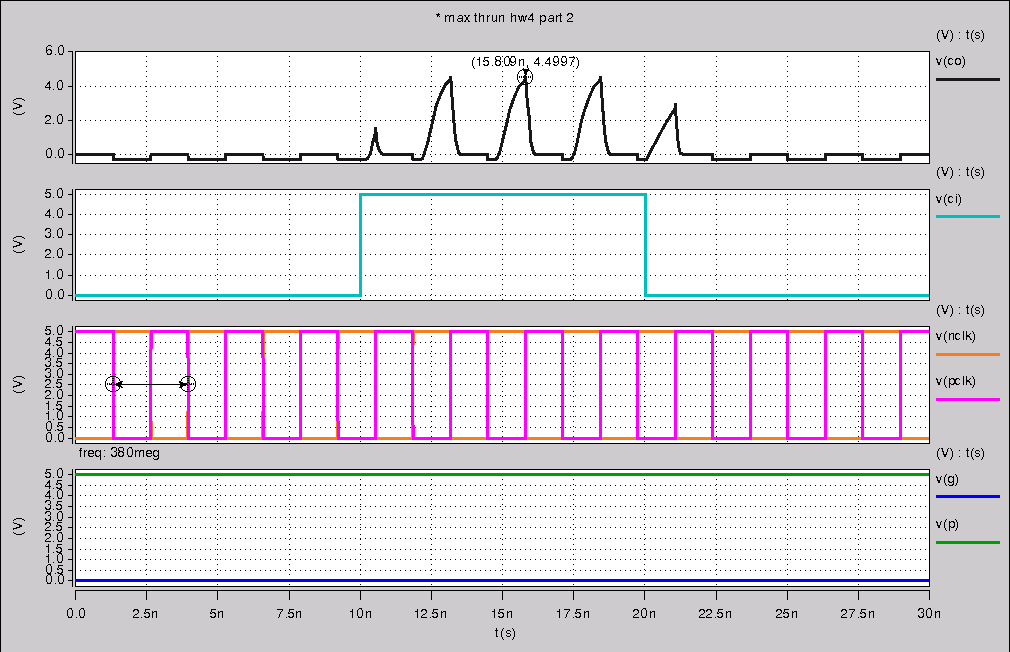
\includegraphics[width=\linewidth]{../part_2_fast.png}
    \caption{Part 2 Simulation Result (Max Clock Speed)}
\end{figure}

\newpage
\subsection*{Part 3}

\lstinputlisting[caption=Part 3 Spice File]{../part_3.sp}

\begin{figure}[H]
    \centering
    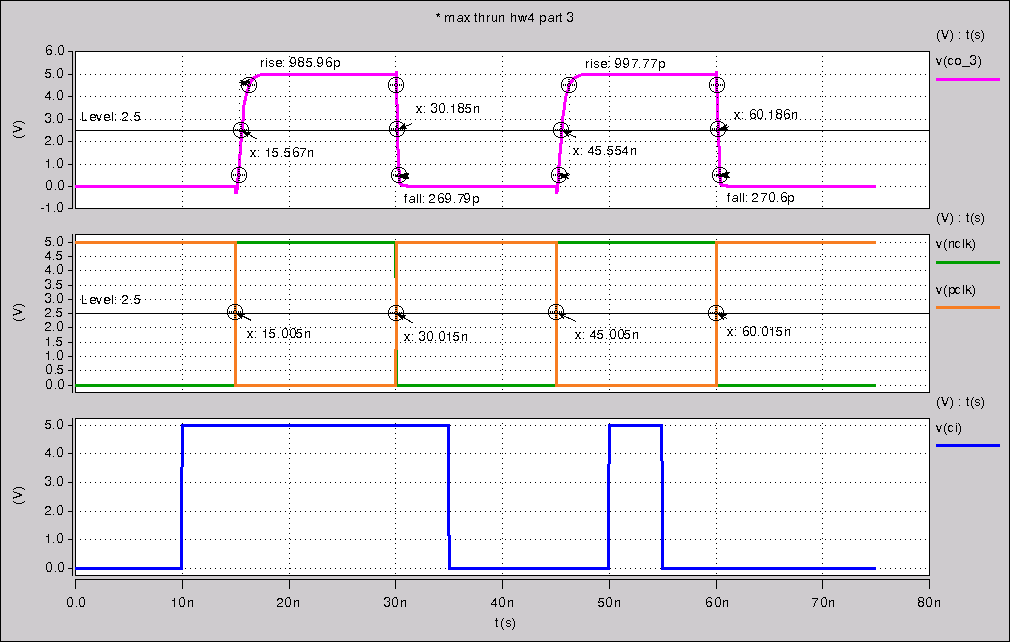
\includegraphics[width=\linewidth]{../part_3.png}
    \caption{Part 3 Simulation Result}
\end{figure}

\begin{figure}[H]
    \centering
    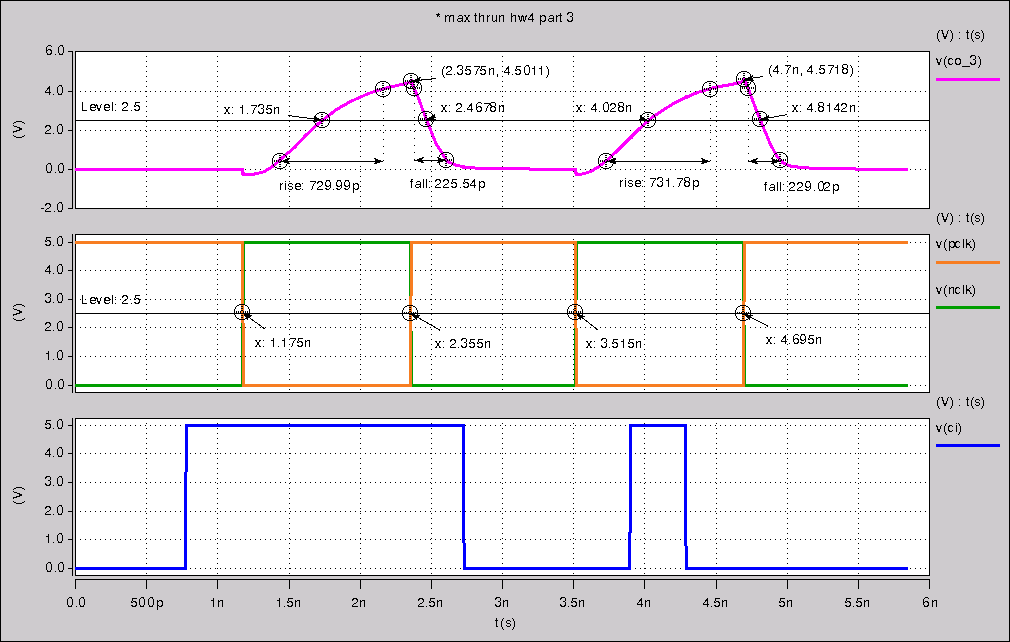
\includegraphics[width=\linewidth]{../part_3_fast.png}
    \caption{Part 3 Simulation Result (Max Clock Speed)}
\end{figure}

\newpage
\subsection*{Part 4}

\lstinputlisting[caption=Part 4 Spice File]{../part_4.sp}

\begin{figure}[H]
    \centering
    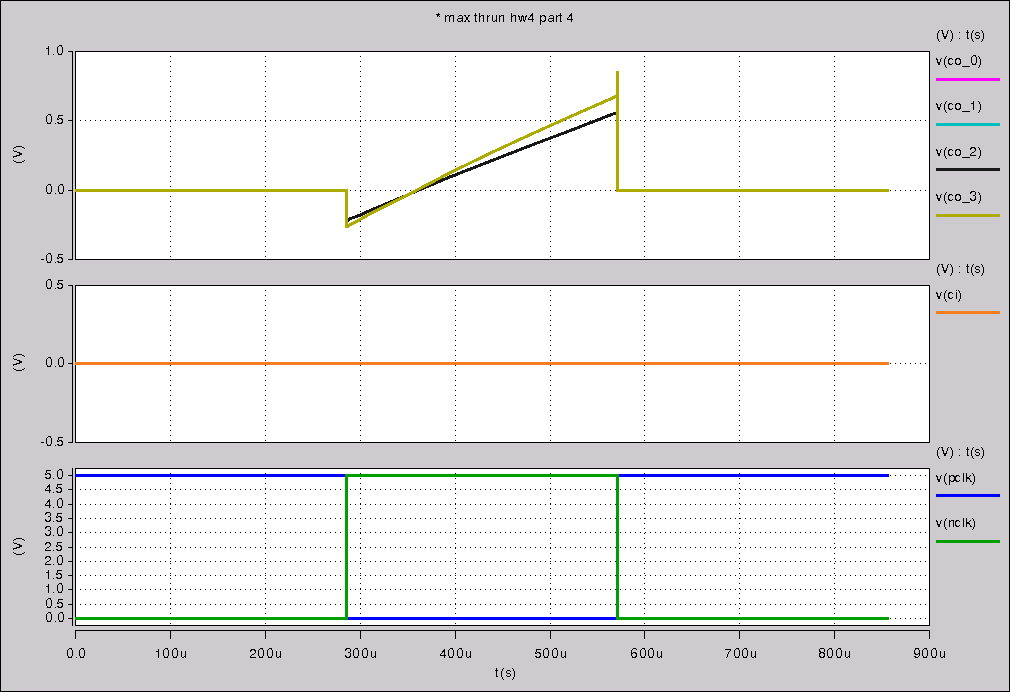
\includegraphics[width=\linewidth]{../part_4.png}
    \caption{Part 4 Simulation Result}
\end{figure}


\begin{table}[H]
    \centering
    \begin{tabular}{cl}
        \toprule
        \textbf{Task} & \textbf{Person}\\
        \midrule
        Part 1 & Qi \\
        Part 2 & Thrun \\
        Part 3 & Both \\
        Part 4 & Qi \\
        Part 5 & Thrun \\
        Part 6 & Qi (with Thrun input on conclusion)\\
        \bottomrule
    \end{tabular}
    \caption{Task Assignment}
\end{table}

\end{document}
